\chapter{Технологическая часть}
\section{Выбор средств программной реализации}
В качестве языка программирования была выбрана Python, ввиду нескольких причин.
\begin{itemize}[label = ---]
    \item Расширенная библиотека стандартных модулей и сторонние библиотеки: Python предоставляет широкий спектр встроенных модулей и сторонних библиотек, которые облегчают разработку компилятора. В частности, библиотеки для парсинга (например, PLY) и работы с абстрактными синтаксическими деревьями (AST) делают разработку компилятора более простой и быстрой.
    \item Простота и читаемость кода: Python известен своей простотой и читаемостью, что особенно важно при разработке и поддержке сложных проектов, таких как компиляторы. Это позволяет легче понимать и изменять код, что сокращает время разработки и уменьшает количество ошибок.
    \item Динамическая типизация и быстрые прототипы: Python поддерживает динамическую типизацию, что позволяет быстрее создавать прототипы и тестировать новые идеи. Это особенно полезно на ранних стадиях разработки компилятора.
    \item Накопленный опыт и существующий код: На момент реализации уже был накоплен существенный опыт в использовании Python, а также существующий код, который можно было использовать и адаптировать для нового проекта. Это существенно сократило бы время и затраты на обучение и разработку.
    \item Кросс-платформенность: Python работает на различных операционных системах, включая Windows, macOS и Linux, что делает его универсальным инструментом для разработки кросс-платформенных приложений.
\end{itemize}
\clearpage
\section{Сгенерированные классы анализаторов}
В результате работы ANTLR генерируются следующие файлы.
\begin{enumerate}
    \item \underline{Oberon.interp} и \underline{OberonLexer.interp} содержат данные (таблицы предсказания, множества следования, информация о правилах грамматики и т.д.) для интерпретатора ANTLR, используются для ускорения работы сгенерированного парсера для принятия решений о разборе входного потока.
    \item \underline{Oberon.tokens} и \underline{OberonLexer.tokens} перечислены символические имена токенов, каждому из которых сопоставлено числовое значение типа токена. ANTLR4 использует их для создания отображения между символическими именами токенов и их числовыми значениями.
    \item Основные модули для компиляции и исполнения в папках сompiler и global\_ops, где папка compile отвечает за инициализацию, декодирование и запуск модулей, а папка global\_ops содержит константы, классы и функции для работы с объектами, типами и инструкциями.   
    \item Папка complier cодержит файл с функциями:
    \begin{itemize}[label = ---]
        \item Compile() – основной процесс компиляции включает в себя инициализацию исходного модуля и запуск модуля. Используется библиотека OSS для инициализации модуля и библиотека OSP для запуска процесса компиляции.
        \item Decode() – функция для декодирования инструкций. Используется библиотека OSG.
        \item Load() – функция для загрузки модуля. Проверяет наличие ошибок перед загрузкой, если ошибок нет и модуль ранее не был загружен, загружает модуль используя библиотеку OSG, а также обновляет состояние переменной loaded.
        \item Exec(S) – функция для выполнения декодированных инструкций. Использует библиотеку OSG.
    \end{itemize}
    \item Папка global\_ops cодержит файл с классами и функциями:
    \begin{itemize}[label = ---]
        \item \textbf{Item} – класс для описания элементов с различными полями, такими как режим, уровень, тип данных, адрес, и другие характеристики.
        \item \textbf{ObjDesc} – класс для описания объектов с различными свойствами, такими как класс объекта, уровень вложенности, следующий объект в цепочке, тип объекта, имя и значение.
        \item \textbf{TypeDesc} – класс для описания типов данных, которые включают форму данных, поля, базовый тип, размер и длину.
        \item Глобальные переменные, такие как intType, boolType, curlev, pc, и массивы для хранения разметки и инструкций:
        \begin{itemize}[label = +]
            \item intType, boolType – указатели на структуры описания типов для целых чисел и булевых значений.
            \item curlev, pc, relx, cno – переменные для отслеживания текущего уровня вложенности, счётчика программ, указателя на текущую команду, и счётчика команд.
            \item regs – множество используемых регистров.
            \item code – массив для хранения кодов инструкций.
            \item rel – массив для хранения информации о относительных адресах.
            \item comname, comadr – массивы для хранения имён и адресов команд.
        \end{itemize}
        \item Функции для работы с регистрами, генерации инструкций и обработки операций:
        \begin{itemize}[label = +]
            \item IncLevel(n) – увеличивает текущий уровень вложенности на заданное значение.
            \item MakeConstItem(x, Type, val) – создает элемент-константу с заданным типом и значением.
            \item MakeItem(x, y) – создает элемент на основе описания объекта.
            \item Field(x, y) – обновляет элемент на основе поля объекта.
            \item Index(x, y) – обновляет элемент на основе индексации массива.
            \item Open() – начальная инициализация глобальных переменных, таких как уровень вложенности и счётчик программ.
            \item Close(S, globals) – завершение процедуры, включающее финальные инструкции (например, возврат из функции).
            \item GetReg(r) – получение свободного регистра.
            \item Put(op, a, b, c) – генерация инструкции с заданными операцией и аргументами.
            \item TestRange(x) – проверка значения на допустимый диапазон.
            \item Header(size) – создание заголовка в коде из указанных размеров.
            \item Enter(size) – функция для входа в новую процедуру с указанием размера области.
            \item EnterCmd(name) – сохранение команды с заданным именем.
        \end{itemize}
    \end{itemize} 
    \item Папка constants содержит все константы.
    \item Папка processor содержит все опепаторы.
    \item Папка file\_io содержит функции работы с файлами. 
    \item Папка keywords содержит все ключевые слова языка Oberon.
    \item Папка output\_executable содержит результат программы.
\end{enumerate}

Таким образом, представленные модулю предоставляют полный набор средств для компиляции и выполнения кода на языке Oberon, включая инициализацию, декодирование, загрузку, выполнение инструкций, а также управление параметрами компиляции и выполнения программ.

\section{Тестирование}

Для проверки корректной работы программы был написан класс TestMethod в файле test.py, который наследуется от unittest.TestCase. В этом классе определены методы для тестирования различных функций компилятора. Тесты используют файл с исходным кодом программы на языке Oberon, находящийся по адресу tests/data/source.mod, и проверяют корректность работы компилятора и выполнения скомпилированного кода.

Каждый метод теста начинает с компиляции, декодирования и загрузки исходного файла. Затем вызывается метод Exec() для выполнения конкретной тестовой команды, и результат сравнивается с ожидаемым результатом при помощи метода assertEqual().

\begin{lstlisting}[label = 8, caption = Пример части класса тестирования]
сlass TestMethods(unittest.TestCase):

def test_multiply_procedure(self):
     compiler.Compile(filename="tests/data/source.mod")
     compiler.Decode()
     compiler.Load()
     self.assertEqual(compiler.Exec("Multiply 5 5"), " 0 40 25")
     self.assertEqual(compiler.Exec("Multiply 0 0"), " 0 0 0")
     self.assertEqual(compiler.Exec("Multiply -1 -1"), " -1 -1 0")
     self.assertEqual(compiler.Exec("Multiply 0 -1"), " 0 -1 0")
     self.assertEqual(compiler.Exec("Multiply 1000 9999"), " 0 102389769999000")
\end{lstlisting}

Рисунок \ref{img:3.1} иллюстрирует вывод результатов тестирования.

\captionsetup{justification=centering,singlelinecheck=off}
\begin{figure}[h!]
	\centering
		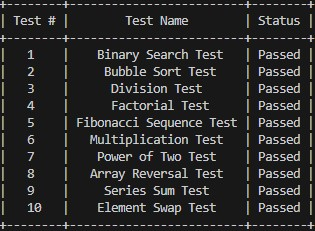
\includegraphics[,scale=1.5]{./img/3.1.jpg}
		\caption{Вывод результатов тестирования.}  
		\label{img:3.1}
\end{figure}